\documentclass[article,shortnames, nojss]{jss}\usepackage[]{graphicx}\usepackage[]{color}
%% maxwidth is the original width if it is less than linewidth
%% otherwise use linewidth (to make sure the graphics do not exceed the margin)
\makeatletter
\def\maxwidth{ %
  \ifdim\Gin@nat@width>\linewidth
    \linewidth
  \else
    \Gin@nat@width
  \fi
}
\makeatother

\usepackage{Sweave}


\usepackage{graphicx, color, amsmath, amssymb, bm, thumbpdf}
%\VignetteEngine{knitr::knitr}

%\VignetteIndexEntry{Parameterization of copula functions}

%\VignetteKeyword{copula}
%\VignetteKeyword{Clayton}
%\VignetteKeyword{Palckett}
%\VignetteKeyword{Hougaard}
%\VignetteKeyword{Poisson}
%\VignetteKeyword{GLM}
%\VignetteKeyword{auxiliary Poisson model}
%\VignetteKeyword{poissonize}
%\VignetteKeyword{data poissonization}
%\VignetteKeyword{surrogate endpoint}
%\VignetteKeyword{surrogate}
%\VignetteKeyword{prediction}
%\VignetteKeyword{leave-one-out}
%\VignetteKeyword{leave-one-trial-out}
%\VignetteKeyword{loocv}
%\VignetteKeyword{cross-validation}
%\VignetteKeyword{clinical trials}
%\VignetteKeyword{random effects}
%\VignetteKeyword{mixed models}


\makeatletter
\def\maxwidth{ %
  \ifdim\Gin@nat@width>\linewidth
    \linewidth
  \else
    \Gin@nat@width
  \fi
}
\makeatother


\usepackage{amsmath, amssymb, bm, thumbpdf}
%%%%%%%%%%%%%%%%%%%%%%%%%%%%%%
%% declarations for jss.cls %%%%%%%%%%%%%%%%%%%%%%%%%%%%%%%%%%%%%%%%%%
%%%%%%%%%%%%%%%%%%%%%%%%%%%%%%

%% almost as usual
\author{
  % Federico Rotolo\\Gustave Roussy\\INSERM U1018 \And
  % Xavier Paoletti\\Gustave Roussy\\INSERM U1018 \And 
  % Marc Buyse\\Universiteit Hasselt\\IDDI\AND
  % Tomasz Burzykowski\\Universiteit Hasselt\\IDDI \And 
  % Stefan Michiels\\Gustave Roussy\\INSERM U1018
}
\title{\pkg{surrosurv}: an \proglang{R} Package for the Evaluation of Failure Time Surrogate Endpoints in Individual Patient Data Meta-Analyses of Randomized Clinical Trials}

\Plainauthor{
  % Federico Rotolo, Xavier Paoletti, Tomasz Burzykowsi, 
  % Marc Buyse, Stefan Michiels
}
\Plaintitle{surrosurv:
            an R Package for the Evaluation of Failure Time Surrogate Endpoints
            in Individual Patient Data Meta-Analyses of Randomized Clinical Trials}
\Shorttitle{\pkg{surrosurv}: Evaluation of Failure Time Surrogate Endpoints in \proglang{R}} 

%% an abstract and keywords
\Abstract{
  Surrogate endpoints are endpoints which are attractive for use in clinical trials
  instead of well-established endpoints because of practical convenience.
  Two measures of surrogacy can be obtained in a meta-analytic context:
  the individual-level $R^2_\text{indiv}$
  and the trial-level $R^2_\text{trial}$.
  % 
  In the case of failure time endpoints,
  the usual two-step approach estimates 
  a Kendall's $\tau$ at the individual level using a copula model,
  and then computes the $R^2_\text{trial}$ via a weighted regression.
  Recently, we also developped an approach based on bivariate survival models with
  individual random effects to measure the $\tau$ and
  treatment-by-trial interactions to measure the $R^2_\text{trial}$.
  We used auxiliary mixed Poisson models to fit such a model.
  
  The \proglang{R} package \pkg{surrosurv} implements the two-step method
  with Clayton, Plackett, and Hougaard copulas
  (with and without measurement-error adjustment),
  as well as the mixed Poisson approach.
  In this paper, we present the package and we show its use in practice
  on individual patient data from a meta-analysis of 4069 patients with advanced/recurrent
  gastric cancer from 20 trials of chemotherapy.
}

\Keywords{surrogate endpoint,
          survival,
          time-to-event,
          randomized clinical trials,
          individual patient data meta-anaysis,
          copula,
          mixed proportional hazard models,
          Poisson regression,
          \pkg{surrosurv},
          \proglang{R}}
\Plainkeywords{surrogate endpoint,
              randomized clinical trials, 
              individual patient data meta-anaysis, 
              copula,
              mixed proportional hazard models,
              Poisson regression,
              surrosurv, 
              R}


%% publication information
%% NOTE: Typically, this can be left commented and will be filled out by the technical editor
%% \Volume{50}
%% \Issue{9}
%% \Month{June}
%% \Year{2012}
%% \Submitdate{2012-06-04}
%% \Acceptdate{2012-06-04}

%% The address of (at least) one author should be given
%% in the following format:
\Address{
  Federico Rotolo, Xavier Paoletti, and Stefan Michiels\\[.4em]
  Service de Biostatistique et d'\'Epid\'emiologie, Gustave Roussy\\
  INSERM U1018 OncoStat, CESP\\
  114, Rue Edouard Vaillant -- Villejuif, F-94805, France\\
  E-mail: \email{federico.rotolo@gustaveroussy.fr}\\
  % 
  % Marc Buyse and Tomasz Burzykowski\\[.4em]
  % I-BioStat, Universiteit Hasselt\\
  % Agoralaan building D --
  % Diepenbeek, B-3590, Belgium\\[.4em]
  % International Drug Development Institute (IDDI)\\
  % Avenue Provinciale 30 --
  % Louvain-la-Neuve, B-1348, Belgium
}
%% Telephone: +43/512/507-7103
%% Fax: +43/512/507-2851

%% for those who use Sweave please include the following line (with % symbols):
%% need no \usepackage{Sweave.sty}

%% end of declarations %%%%%%%%%%%%%%%%%%%%%%%%%%%%%%%%%%%%%%%%%%%%%%%
\IfFileExists{upquote.sty}{\usepackage{upquote}}{}
\begin{document}

% \SweaveOpts{prefix.string=figs/fig}
% \SweaveOpts{height=4}
% \SweaveOpts{width=7}
% \setkeys{Gin}{width=\textwidth}
% \SweaveOpts{concordance=FALSE}
%% Use the \pkg{}, \proglang{} and \code{} commands.

%%%%%%%%%%%%%%%%%%%%%%%%%%%%%%%%%%%%%%%%%%%%%%%%%%%%%%%%%%%%%%%%%%%%%%%%%%%%%%%%
%%%%%%%%%%%%%%%%%%%%%%%%%%%%%%%%%%%%%%%%%%%%%%%%%%%%%%%%%%%%%%%%%%%%%%%%%%%%%%%%
%%%%%%%%%%%%%%%%%%%%%%%%%%%%%%%%%%%%%%%%%%%%%%%%%%%%%%%%%%%%%%%%%%%%%%%%%%%%%%%%
\section{Introduction}
%%%%%%%%%%%%%%%%%%%%%%%%%%%%%%%%%%%%%%%%%%%%%%%%%%%%%%%%%%%%%%%%%%%%%%%%%%%%%%%%
%%%%%%%%%%%%%%%%%%%%%%%%%%%%%%%%%%%%%%%%%%%%%%%%%%%%%%%%%%%%%%%%%%%%%%%%%%%%%%%%
%%%%%%%%%%%%%%%%%%%%%%%%%%%%%%%%%%%%%%%%%%%%%%%%%%%%%%%%%%%%%%%%%%%%%%%%%%%%%%%%

Surrogate endpoints are endpoints which can reliably used
  instead of well-established endpoints
  and which yield improved practical convenience
  in terms of cost, rapidity or ease of assessment, 
  or reduced invasiveness \citep{Burzykowski2006}.
A reliable surrogate endpoint must be strongly associatied with
  the true endpoints at the individual level and
  the effect of the treatment on the surrogate
  must be assciated with the effect on the true endpoint.
In a meta-analytic context,
  the usual measure of individual level surrogacy for continuous endpoints is
  the $R^2_\text{\tiny indiv}$ 
  and the ususal measure of trial level surrogacy
  is the  $R^2_\text{\tiny trial}$ \citep{BuyseEtal00}.

In the case of failure time (survival) endpoints,
  the classical methods developped for normally-distributed endpoints
  cannot be used because of right censoring.
\cite{BurzykowskiEtal01} proposed a meta-analytic model
  for failure time endpoints that measures
  individual level surrogacy in terms of \cite{Kendall38}'s $\tau$
  and trial level surrogacy in terms of $R^2_\text{\tiny trial}$.
Despite the numerous applications of this approach in the medical literature,
  difficults exists to fit the whole model directly and
  a two-step procedure is commonly employed.
Such a procedure has some limitations 
  preventing its applicability in a number of applications,
  including convergence issues which can make the interpretation of the results difficult
  \citep{Oba2013, BurzykowskiCortinas05}.
In principle, the most natural framework for adapting the meta-analytic approach
  by \cite{BuyseEtal00} to the survival case
  is the use of bivariate mixed proportional hazard models,
  also known as frailty models \citep{DuchateauJanssen08}.
Since the estimation of frailty models with complex structures
  of random effects is computationally intensive and can fail to converge,
  we previously exploited \citep{RotoloPoissurogate}
  the well-known connection between the proportional hazard models
  and the Poisson log-linear models  \citep{Whitehead80, LairdOlivier81},
  which has also been used more recently for individual patient data meta-analyses
  \citep{crowtherEtal12}.

In the present paper, we show how all these models can be fitted by use 
  of the \proglang{R} \citep{R}
  package \pkg{surrosurv} \citep{R:surrosurv}.
We illustrate the use of the available functions 
  using individual data of a meta-analysis of 20 randomized trials of chemotherapy,
  including 4069 patients with advanced/recurrent gastric cancer
  \citep{GASTRIC13, Paoletti2013}.


%%%%%%%%%%%%%%%%%%%%%%%%%%%%%%%%%%%%%%%%%%%%%%%%%%%%%%%%%%%%%%%%%%%%%%%%%%%%%%%%
%%%%%%%%%%%%%%%%%%%%%%%%%%%%%%%%%%%%%%%%%%%%%%%%%%%%%%%%%%%%%%%%%%%%%%%%%%%%%%%%
%%%%%%%%%%%%%%%%%%%%%%%%%%%%%%%%%%%%%%%%%%%%%%%%%%%%%%%%%%%%%%%%%%%%%%%%%%%%%%%%
\section{The evaluation of failure time surrogate endpoints}
\label{sec:methods}
%%%%%%%%%%%%%%%%%%%%%%%%%%%%%%%%%%%%%%%%%%%%%%%%%%%%%%%%%%%%%%%%%%%%%%%%%%%%%%%%
%%%%%%%%%%%%%%%%%%%%%%%%%%%%%%%%%%%%%%%%%%%%%%%%%%%%%%%%%%%%%%%%%%%%%%%%%%%%%%%%
%%%%%%%%%%%%%%%%%%%%%%%%%%%%%%%%%%%%%%%%%%%%%%%%%%%%%%%%%%%%%%%%%%%%%%%%%%%%%%%%

Let $T_{ij}$ and $S_{ij}$ be the times to the true and the surrogate 
  endpoints, respectively,
  for patient $j\in\{1, \ldots, n_i\}$
  in trial  $i\in\{1, \ldots, N\}$.
Let $Z_{ij}$ be the indicator of the treatment arm
  to which the $j$-th patient in the $i$-th trial has been randomized.


%%%%%%%%%%%%%%%%%%%%%%%%%%%%%%%%%%%%%%%%%%%%%%%%%%%%%%%%%%%%%%%%%%%%%%%%%%%%%%%%
%%%%%%%%%%%%%%%%%%%%%%%%%%%%%%%%%%%%%%%%%%%%%%%%%%%%%%%%%%%%%%%%%%%%%%%%%%%%%%%%
\subsection{Two-step copula approach}
%%%%%%%%%%%%%%%%%%%%%%%%%%%%%%%%%%%%%%%%%%%%%%%%%%%%%%%%%%%%%%%%%%%%%%%%%%%%%%%%
%%%%%%%%%%%%%%%%%%%%%%%%%%%%%%%%%%%%%%%%%%%%%%%%%%%%%%%%%%%%%%%%%%%%%%%%%%%%%%%%
\label{sec:copulaApp}
The model proposed by \cite{BurzykowskiEtal01} for failure time endpoints
  consists in two steps, one for the individual and one for the trial level.

\paragraph{Individual-level.}
At the first the bivariate proportional hazard model is defined
  by means of the marginal hazard functions and the copula function
  accounting for their dependence:
  \begin{equation}
    \begin{cases}
      h_{Sij}(s; Z_{ij}) = h_{Si}(s) \exp\big\{
        \alpha_i Z_{ij} 
      \big\}\\
      h_{Tij}(t; Z_{ij}) = h_{Ti}(t) \exp\big\{
        \beta_i Z_{ij}
      \big\}\\
      C_\theta(S_{Sij}(s), S_{Tij}(t))
    \end{cases}
    \label{eq:copulaModel}
  \end{equation}
  where $h_{Si}(s)$ and $h_{Ti}(s)$ are the trial-specific baseline hazards,
  $\alpha_i$ and $\beta_i$ the treatment effects,
  and $S_{Sij}(s)$ and $S_{Tij}(t)$ the survival functions associated to
  of $h_{Tij}$ and $h_{Tij}$.
The dependence parameter $\theta$
  is reparametrized into the individual-level Kendall's $\tau$,
  according to the copula function
  thanks to the \code{tau()} function in the 
  \pkg{copula} package \citep{R:copula, Yan07}.

In the \pkg{surrosurv} package,
  Weibull marginal hazards are implemented,
  together with three copula functions:
  \begin{itemize}
    \item the \cite{Clayton78} copula
      \begin{equation}
        C_\theta(u, v)= \left(u^{-\theta} + v^{-\theta} - 1\right)^{-1/\theta},
        \label{eq:clayton}
      \end{equation}
      with $\theta > 0$
      and Kendall's $\tau = \theta/(\theta+2)$;
    \item the \cite{Plackett65} copula
      \begin{align}
        C_\theta(u,v) &= \big[ Q - R^{1/2} \big] / \big[2 (\theta - 1) \big],\\
        Q &= 1 +(\theta-1)(u+v), \nonumber\\
        R &= Q^2 - 4 \theta(\theta-1)uv, \nonumber
      \end{align}
      with $\theta > 0$ and Kendall's $\tau$ computed numerically
      as no analytical expression is available;
    \item the \cite{Hougaard86} copula
      \begin{equation}
        C_\theta(u,v) = \exp\left(-\left[(- \ln u)^{1/\theta} +
        (- \ln v)^{1/\theta}\right]^\theta \right),
      \end{equation}
      with $\theta \in (0, 1)$ 
      and Kendall's $\tau = 1 - \theta$.
  \end{itemize}
Further details on these three copula models can be found in the 
  \code{vignette(}\verb|'|\code{copula}\verb|'|\code{, package =}
  \verb|'|\code{surrosurv}\verb|')|.

\paragraph{Trial level.}
At the second step, the estimates of the treatment effects 
  obtained at the first step are assumed to follow the mixed model
  \begin{align}
    \left(\begin{array}{c} 
      {\hat\alpha_i}\\ {\hat\beta_i}\end{array}\right)
    &= \left(\begin{array}{c} \alpha_i\\ \beta_i\end{array}\right) +
      \left(\begin{array}{c} \epsilon_{ai}\\ \epsilon_{bi}\end{array}\right),
    \\
    \left(\begin{array}{c} {\alpha_i}\\ {\beta_i}\end{array}\right)
    & \sim \mathcal N
      \left(
      \left(\begin{array}{c}
      \alpha\\ \beta\end{array}\right), 
      \bm D = \left(\begin{array}{cc} 
      d_a^2 &
      d_a d_b{\rho_\text{\tiny trial}} \\
      d_a d_b{\rho_\text{\tiny trial}} &
      d_b^2 \\
      \end{array}\right)
      \right),
      \label{eq:trtEffs}
    \\
    \left(\begin{array}{c} \epsilon_{ai}\\ \epsilon_{bi}\end{array}\right)
    &\sim \mathcal N \left(
      \left(\begin{array}{c}0\\0\end{array}\right),
      \bm\Omega_i = \left(\begin{array}{cc} 
            \omega_{ai}^2 &
            \omega_{ai} \omega_{bi} {\rho_{\epsilon i}} \\
            \omega_{ai} \omega_{bi} {\rho_{\epsilon i}} &
            \omega_{bi}^2 \\
        \end{array}\right)\right).
  \end{align}
  where $(\alpha_i, \beta_i)^\prime$ are the true treatment effects
  and $(\epsilon_{ai}, \epsilon_{bi})^\prime$ the estimation errors.

The trial-level surrogacy measure is
  $R_\text{\tiny trial}^2 = \rho_\text{\tiny trial}^2$.
In practice, the $\rho_\text{\tiny trial}$ is computed
  via a linear regression of the $\beta_i$'s over the $\alpha_i$'s
  adjusted by measurement error by fixing the $\bm\Omega_i$'s at their estimates
  from the first step \citep{vanHouwelingenEtal02}
  by using the \pkg{mvmeta} package \citep{GasparriniEtal12, R:mvmeta}.
This adjusted (for measurement error) model is sometimes computationally challenging
  and does not always converge.
The \pkg{surrosurv} package returns also the so-called
  unadjusted $R_\text{\tiny trial}^2$,
  obtained using a linear regression ---
  equivalent to fixing all the elements of $\bm\Omega_i$ equal to 0 ---
  by weigthing the observations $(\alpha_i, \beta_i)^\prime$ by the trial size,
  in order to account somehow indirectly and approximately for measurement error.



%%%%%%%%%%%%%%%%%%%%%%%%%%%%%%%%%%%%%%%%%%%%%%%%%%%%%%%%%%%%%%%%%%%%%%%%%%%%%%%%
%%%%%%%%%%%%%%%%%%%%%%%%%%%%%%%%%%%%%%%%%%%%%%%%%%%%%%%%%%%%%%%%%%%%%%%%%%%%%%%%
\subsection{One-step mixed Poisson approach}
%%%%%%%%%%%%%%%%%%%%%%%%%%%%%%%%%%%%%%%%%%%%%%%%%%%%%%%%%%%%%%%%%%%%%%%%%%%%%%%%
%%%%%%%%%%%%%%%%%%%%%%%%%%%%%%%%%%%%%%%%%%%%%%%%%%%%%%%%%%%%%%%%%%%%%%%%%%%%%%%%

Let us assume that the bivariate proportional hazard model given by the first
  two lines of equation (\ref{eq:copulaModel}) holds conditionally
  on an individual random effect
  $u_{ij} \sim \mathcal N(0, \sigma^2_\text{\tiny indiv})$:
  \begin{equation}
    \begin{cases}
      h_{Sij}(s\mid u_{ij}) = h_{S i}(s)
      \exp\left\{u_{ij} + \alpha_i Z_{ij} \right\}\\
      h_{Tij}(t\mid u_{ij}) = h_{T i}(t)
      \exp\left\{u_{ij} + \beta_i Z_{ij}\right\}.
    \end{cases}
    \label{eq:biHaz}
  \end{equation}
Note that this corresponds to a  shared frailty model with 
  bivariate clusters \citep{DuchateauJanssen08}.
The shared frailty term $u_{ij}$ accounts for individual level dependence.

It is well-known \cite[see for instance][]{Whitehead80, crowtherEtal12}
  that the parameters of Cox models can be estimated by fitting
  a so-called `auxiliary' Poisson log-linear regression model,
  by dividing the time scale into intervals $k=1, \ldots, K$.
The auxiliary Poisson model provides the same estimator as the Cox model
  if the bounds of the intervals are all the observed event times,
  and an approximation of the Cox estimators otherwise.
In the surrogacy assessment context,
  the parameters of the bivariate frailty model (\ref{eq:biHaz})
  can be estimated via a bivariate mixed Poisson model
  \begin{equation}
    \begin{cases}
      \log\left( \mu_{S ij}^{(k)} \right) = 
        \mu_{S i}^{(k)}  + u_{ij}
        + \alpha_i Z_{ij}
        + \log\left(y_{S ij}^{(k)} \right)\\
      \log\left( \mu_{T ij}^{(k)} \right) = 
        \mu_{T i}^{(k)}  + u_{ij}
        + \beta_i Z_{ij}
        + \log\left(y_{T ij}^{(k)} \right)
    \end{cases}
    \label{eq:biPoiMix}
  \end{equation}
  with $y_{Sj}^{(k)}$ and $y_{Tj}^{(k)}$ the time spent at risk
  by subject $i$ in trial $j$ for each endpoint
  during the period $k$.


%%%%%%%%%%%%%%%%%%%%%%%%%%%%%%%%%%%%%%%%%%%%%%%%%%%%%%
\paragraph{Individual-level surrogacy.}
%%%%%%%%%%%%%%%%%%%%%%%%%%%%%%%%%%%%%%%%%%%%%%%%%%%%%%
The use of the a shared frailty $u_{ij}$,
the estimated variance of which  is $\hat\sigma^2_\text{\tiny indiv}$,
can be used to compute an estimate of the Kendall's
$\hat\tau = 4 \int_0^\infty s \mathcal L(s)\mathcal L^{(2)}(s) \textrm d s - 1$,
where $\mathcal L(s)$ and $\mathcal L^{(2)}(s)$
are the Laplace transform of the frailty distribution and its
second derivative.
As an analytic expression of $\mathcal L(s)$
is not available for the log-normal frailty distribution,
we approximated it using the Laplace method \citep{GoutisCasella99},
implemented in the \code{fr.lognormal()} function
in the \pkg{parfm} package \citep{parfmJSS, R:parfm}.


%%%%%%%%%%%%%%%%%%%%%%%%%%%%%%%%%%%%%%%%%%%%%%%%%%%%%%
\paragraph{Trial-level surrogacy.} \label{sec:trialDep}
%%%%%%%%%%%%%%%%%%%%%%%%%%%%%%%%%%%%%%%%%%%%%%%%%%%%%%
In model (\ref{eq:biPoiMix}),
the same assumptions (\ref{eq:trtEffs})
as in the two-step copula model
are done for the trial-specific treatment effects
Thus, the correlation $\rho_\text{\tiny trial}$
between the two treatment effects provides us with 
the coefficient of determination
$R^2_\text{\tiny trial} = \rho^2_\text{\tiny trial}$,
also referred to simply as $R^2$.


%%%%%%%%%%%%%%%%%%%%%%%%%%%%%%%%%%%%%%%%%%%%%%%%%%%%%%
\paragraph{Reduced Poisson models.}
%%%%%%%%%%%%%%%%%%%%%%%%%%%%%%%%%%%%%%%%%%%%%%%%%%%%%%
In order to deal with convergence issues,
the \pkg{surrosurv} package computes four reduced versions 
of the full model (\ref{eq:biPoiMix}).
\begin{itemize}
\item Model \textbf{Poisson T} has
random trial-treatment interactions $\alpha_i$ and $\beta_i$,
but does not incoroporate individual effects ($u_{ij} \equiv 0$)
and it has common baselines between trials
($\mu^{(k)}_{Si} = \mu^{(k)}_{S}$, $\mu^{(k)}_{Ti} = \mu^{(k)}_{T},
\forall i$).
This model provides only the trial-level measure of surrogacy
$R^2_{\textsf{\tiny trial}}$.

\item Model \textbf{Poisson I} contains individual random effects $u_{ij}$,
but not the trial-specific treatment effects 
($\alpha_i = \alpha$, $\beta_i = \beta, \forall i$)
and has common baselines between trials.
This model provides only the individual-level measure of surrogacy
$\tau$.

\item Model \textbf{Poisson TI} incorporates
both random trial-treatment interactions
$(\alpha_i, \beta_i)^\prime$
and individual random effects $u_{ij}$,
but still has common baselines between trials.
It provides both individual-level and trial-level measures of surrogacy
$\tau$ and $R^2_{\textsf{\tiny trial}}$.

\item Model \textbf{Poisson TIa} extends the model Poisson TI
by accounting for trial-specific baseline risks,
using shared random effects at the trial level:
$\mu_{Si} = \mu_S + m_i, \mu_{Ti} = \mu_T + m_i$,
with $m_i\sim\mathcal N(0, \sigma^2_m)$.
\end{itemize}



%%%%%%%%%%%%%%%%%%%%%%%%%%%%%%%%%%%%%%%%%%%%%%%%%%%%%%%%%%%%%%%%%%%%%%%%%%%%%%%%
%%%%%%%%%%%%%%%%%%%%%%%%%%%%%%%%%%%%%%%%%%%%%%%%%%%%%%%%%%%%%%%%%%%%%%%%%%%%%%%%
%%%%%%%%%%%%%%%%%%%%%%%%%%%%%%%%%%%%%%%%%%%%%%%%%%%%%%%%%%%%%%%%%%%%%%%%%%%%%%%%
\section[A data example within the surrosurv package]{A data example within the \pkg{surrosurv} package}
%%%%%%%%%%%%%%%%%%%%%%%%%%%%%%%%%%%%%%%%%%%%%%%%%%%%%%%%%%%%%%%%%%%%%%%%%%%%%%%%
%%%%%%%%%%%%%%%%%%%%%%%%%%%%%%%%%%%%%%%%%%%%%%%%%%%%%%%%%%%%%%%%%%%%%%%%%%%%%%%%
%%%%%%%%%%%%%%%%%%%%%%%%%%%%%%%%%%%%%%%%%%%%%%%%%%%%%%%%%%%%%%%%%%%%%%%%%%%%%%%%
We illustrate the use of the function in the \pkg{surrosurv} package
by means of the individual patient data of the advanced GASTRIC meta-analysis
\citep{GASTRIC13, Paoletti2013}.
\begin{Schunk}
\begin{Sinput}
R> library('surrosurv')
\end{Sinput}
\begin{Soutput}
Loading required package: optimx
\end{Soutput}
\begin{Sinput}
R> packageVersion('surrosurv')
\end{Sinput}
\begin{Soutput}
[1] '1.1.4'
\end{Soutput}
\end{Schunk}

The individual data of the 4069 patients,
already made public by \cite{BuyseEtal15},
are also available directly in \proglang{R} in the \pkg{surrosurv} package:
\begin{Schunk}
\begin{Sinput}
R> data('gastadv')
R> nrow(gastadv)
\end{Sinput}
\begin{Soutput}
[1] 4069
\end{Soutput}
\end{Schunk}

The data set contains the following variables:
\begin{Schunk}
\begin{Sinput}
R> names(gastadv)
\end{Sinput}
\begin{Soutput}
[1] "timeT"    "statusT"  "statusS"  "timeS"    "trialref" "trt"      "id"      
\end{Soutput}
\end{Schunk}
where \code{timeT} and \code{timeS} are the (possibly censored) times 
for overall survival (\code{T}) and
for progression-fre survival (\code{S}) expressed in days,
\code{statusT} and \code{statusS} are the associated indicators of
censoring (\code{0}) or event (\code{1}),
\code{trialref} is the trial indicator ($i$),
\code{trt} is the treatment arm (\code{-0.5} for control and \code{0.5} for chemotherapy),
and \code{id} is the patient indicator ($j$).
Figure~\ref{fig:survCurves} shows the survival curves for overall survival,
the true endpoint $T$, and progression-free survival,
the candiddate surrogate $S$.
\begin{Schunk}
\begin{figure}
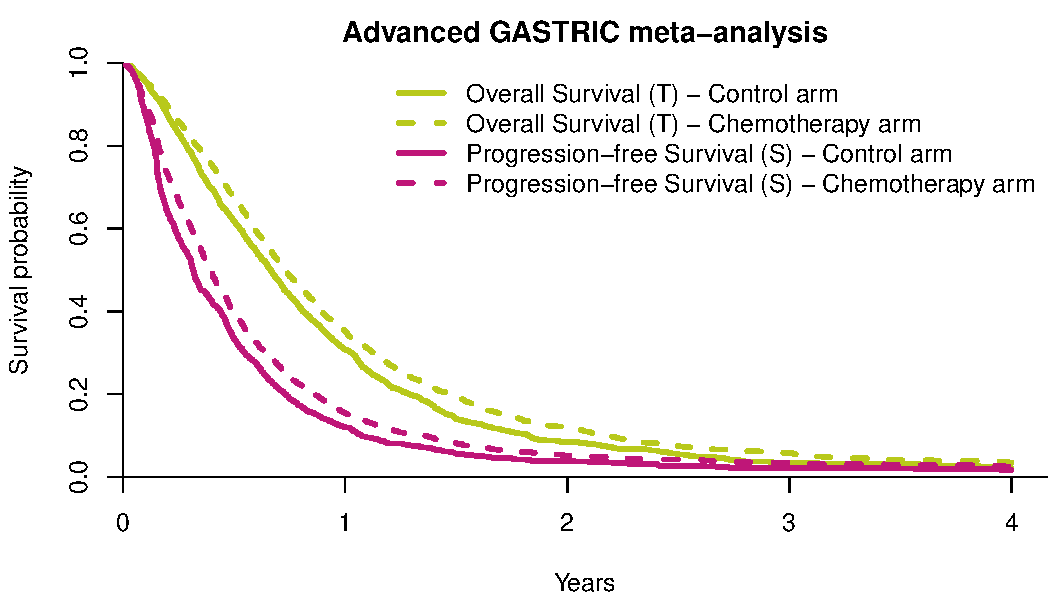
\includegraphics[width=\textwidth]{./survCurves-1} \caption[Survival curves for overall survival ($T$) and progression-free survival $S$ in the advanced GASTRIC meta-analysis \citep{GASTRIC13}]{Survival curves for overall survival ($T$) and progression-free survival $S$ in the advanced GASTRIC meta-analysis \citep{GASTRIC13}}\label{fig:survCurves}
\end{figure}
\end{Schunk}

  
%%%%%%%%%%%%%%%%%%%%%%%%%%%%%%%%%%%%%%%%%%%%%%%%%%%%%%%%%%%%%%%%%%%%%%%%%%%%%%%%
%%%%%%%%%%%%%%%%%%%%%%%%%%%%%%%%%%%%%%%%%%%%%%%%%%%%%%%%%%%%%%%%%%%%%%%%%%%%%%%%
\section{Fitting the surrogacy models}
%%%%%%%%%%%%%%%%%%%%%%%%%%%%%%%%%%%%%%%%%%%%%%%%%%%%%%%%%%%%%%%%%%%%%%%%%%%%%%%%
%%%%%%%%%%%%%%%%%%%%%%%%%%%%%%%%%%%%%%%%%%%%%%%%%%%%%%%%%%%%%%%%%%%%%%%%%%%%%%%%
  The surrogacy models presented in Section~\ref{sec:methods}
  can be fitted via the \code{surrosurv()} function.
  
  The only mandatory argument for the \code{surrosurv()} function is
  \code{data}, which has to be a data.frame with columns
  \begin{itemize}
  \item \code{trialref}, a factor containing the trial identifier;
  \item \code{trt}, the treatment arm, coded as \code{-0.5} \textit{vs.} \code{0.5};
  \item \code{id}, a factor containing the patient id;
  \item \code{timeT} and \code{timeS}, two positive-valued numerical variables,
  containing the observed or censoring times of the true endpoint $T$
  and of the candidate surrogate $S$, respectively;
  \item \code{statusT} and \code{statusS},
  the censoring/event (\code{0}/\code{1}) indicators of $T$ and $S$, respectively.
  \end{itemize}
  
  A second argument, \code{models}, can optionally contain the list of the models to fit.
  It can contain  ny value of 
  \code{clayton}, \code{plackett}, \code{hougaard}, or \code{poisson}).
  If not specified, all of them are fitted.
  
  Two further parameters, \code{intWidth} and \code{nInts},
  specify the width and the number of time intervals for data Poissonization.
  These parameters are passes to the function \code{poissonize()},
  described in the Appendix (Sec.~\ref{sec:poisson}).
  Only one of them can be specified.
  By default, \code{nInts = 8} which means that the study period is divided into
  eight periods, the length of which is fixed so that 1/8th of the observed
  events falls in each interval.
  
  The optimizer used for optimization of the copula models and the Poisson models
  can be passed via the arguments \code{cop.OPTIMIZER} and \code{poi.OPTIMIZER},
  passed to the \pkg{optimx} package \citep{optimxJSS, R:optimx}.
  
  The last parameter, \code{verbose}, is a logical value
  stating whether the function should print out the model being fitted
  (default: \code{FALSE}).
  
  
  The surrogacy models for the advanced GASTRIC cancer meta-analysis
  are obtained as follows:
\begin{Schunk}
\begin{Sinput}
R> allSurroRes <-  surrosurv(gastadv, verbose = TRUE)
\end{Sinput}
\begin{Soutput}
Estimating model: clayton
\end{Soutput}
\begin{Soutput}
Estimating model: plackett
\end{Soutput}
\begin{Soutput}
Estimating model: hougaard
\end{Soutput}
\begin{Soutput}
Estimating model: poisson
\end{Soutput}
\end{Schunk}
Note that, the computation time of the surrogacy models can be long.
In this example, the computations required
  38
  mins
  on a PC with an Intel\textsuperscript{\textregistered} quad-core CPU E3-1280 V2
  with 3.60 GHz clock speed and 16GB of RAM.
The results are an object of class \code{surrosurv}
  and the estimated Kendall's $\tau$ and $R^2$ can be easily shown:
\begin{Schunk}
\begin{Sinput}
R>   allSurroRes
\end{Sinput}
\begin{Soutput}
               kTau R2  
Clayton unadj  0.61 0.45
Clayton adj    0.61 0.42
Plackett unadj 0.62 0.45
Plackett adj   0.62 0.41
Hougaard unadj 0.32 0.45
Hougaard adj   0.32 0.38
PoissonT       -.-- 1   
PoissonI       0.51 -.--
PoissonTI      0.51 0.63
PoissonTIa     0.51 0.83
\end{Soutput}
\end{Schunk}
For each copula model,
  both the results with measurement error adjustment (\code{adj})
  and without adjustment (\code{unadj}) are shown.

\subsection{Assessing convergence}
The function \code{convergence()} checks whether convergence criteria
  are met by each of the fitted models:
\begin{Schunk}
\begin{Sinput}
R>   convergence(allSurroRes)
\end{Sinput}
\begin{Soutput}
               maxSgrad minHev minREev
Clayton unadj     FALSE  FALSE     ---
Clayton adj       FALSE  FALSE    TRUE
Plackett unadj    FALSE  FALSE     ---
Plackett adj      FALSE  FALSE    TRUE
Hougaard unadj    FALSE   TRUE     ---
Hougaard adj      FALSE   TRUE    TRUE
PoissonT           TRUE   TRUE   FALSE
PoissonI           TRUE   TRUE     ---
PoissonTI          TRUE   TRUE    TRUE
PoissonTIa         TRUE   TRUE    TRUE
\end{Soutput}
\end{Schunk}
Three convergence criteria are considered.
The first criterion, \code{maxSgrad},
  verifies whether the maximum gradient is small enough.
The two other criteria, \code{minHev} and \code{minREev},
  verify whether the minimum eigenvalue
  of the Hessian matrix of the fixed parameters (\code{H})
  and of the covariance matrix of the random effects (\code{RE})
  are big enough,
  in order to assure the positive definitess of the two matrices.
Two parameters can be used to tune the thresholds
  for `small enough' maximum gradient and 
  for `big enough' minmum eigen value:
  \code{kkttol} (\code{1e-2} by default),
  and \code{kkt2tol} (\code{1e-8} by default).

If the values of the minimum gradient and of the maximum eigenvalues are needed,
  the function \code{convals()} can be used:
\begin{Schunk}
\begin{Sinput}
R>   convals(allSurroRes)
\end{Sinput}
\begin{Soutput}
               maxSgrad   minHev minREev
Clayton unadj   1.5e+00 -6.1e+00     ---
Clayton adj     1.5e+00 -6.1e+00 9.8e-03
Plackett unadj  4.1e+02 -5.2e+00     ---
Plackett adj    4.1e+02 -5.2e+00 8.7e-03
Hougaard unadj  1.4e+01  7.7e-01     ---
Hougaard adj    1.4e+01  7.7e-01 7.7e-03
PoissonT        1.3e-05  1.3e+02 6.3e-12
PoissonI        2.0e-05  6.8e+01     ---
PoissonTI       7.1e-06  6.7e+01 2.0e-02
PoissonTIa      5.0e-05  9.4e+07 1.0e-01
\end{Soutput}
\end{Schunk}


%%%%%%%%%%%%%%%%%%%%%%%%%%%%%%%%%%%%%%%%%%%%%%%%%%%%%%%%%%%%%%%%%%%%%%%%%%%%%%%%
%%%%%%%%%%%%%%%%%%%%%%%%%%%%%%%%%%%%%%%%%%%%%%%%%%%%%%%%%%%%%%%%%%%%%%%%%%%%%%%%
\section{Prediction of the treatment effect}
%%%%%%%%%%%%%%%%%%%%%%%%%%%%%%%%%%%%%%%%%%%%%%%%%%%%%%%%%%%%%%%%%%%%%%%%%%%%%%%%
%%%%%%%%%%%%%%%%%%%%%%%%%%%%%%%%%%%%%%%%%%%%%%%%%%%%%%%%%%%%%%%%%%%%%%%%%%%%%%%%
When fitting surrogacy models,
  an estimate of the treatment effects on the two endpoints
  is computed internally for each trial.
The function \code{predict()}, applied to an object of class \code{surrosurv},
  returns the treatment effect predictions
  for each trial.
The minimal syntax is \code{predict(allSurroRes)},
  but one can be interested in prediction of only one of the fitted models:
\begin{Schunk}
\begin{Sinput}
R>   predict(allSurroRes, models = 'PoissonTI')
\end{Sinput}
\begin{Soutput}
Treatment effect prediction for surrosurv object

   Poisson TI 
                            1     2     3     4     5     6        
    Treatment effects on S: -0.52 -0.42 -0.38 -0.08 -0.51 -0.38 ...
    Treatment effects on T: -0.26 -0.08 -0.27  0.41 -0.41 -0.15 ...
\end{Soutput}
\end{Schunk}
This function returns an object of class \code{predictSurrosurv}.

The predicted treatment effects can also be vizualied graphically
  using the linear regression of the effect on $T$ given the effect on $S$.
The usual surrogacy plot is obtained using the function \code{plot()}
  for the classes \code{surrosurv} and \code{predictSurrosurv}.
For example, the surrogacy plots
  for the adjusted Clayton copula and the Poisson TI models
  in the advanced GASTRIC meta-analysis (Fig.~ref{fig:predictions})
  can be obtained as follows:
\begin{Schunk}
\begin{figure}
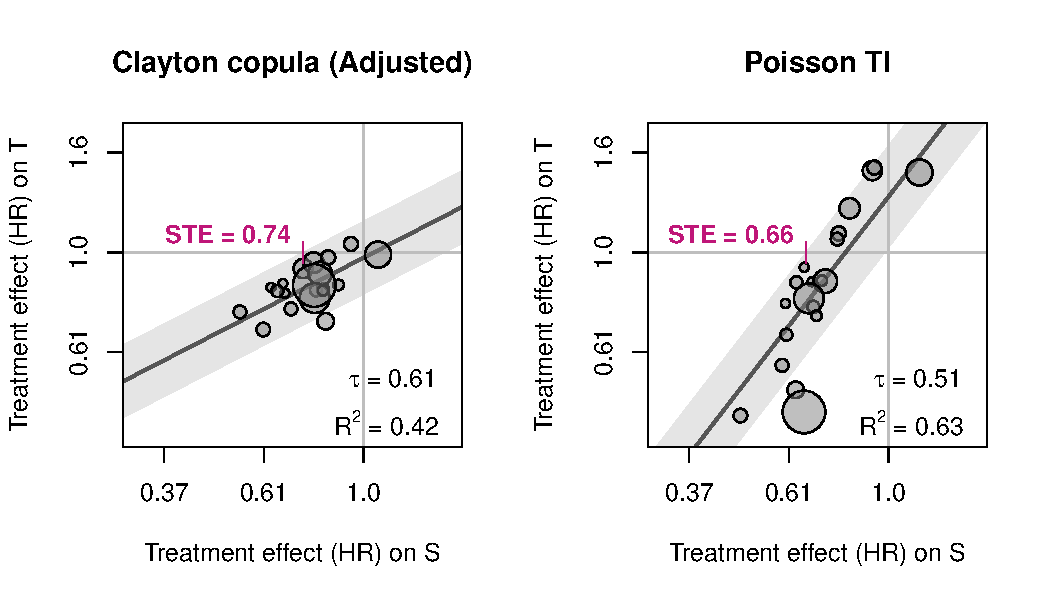
\includegraphics[width=\textwidth]{./predictions-1} \caption[Predictions for the advanced GASTRIC meta-analysis \citep{GASTRIC13}, as computed by the adjusted Clayton copula model, which had poor convergence metrics, and by the Poisson TI model, which was deemed to have converged]{Predictions for the advanced GASTRIC meta-analysis \citep{GASTRIC13}, as computed by the adjusted Clayton copula model, which had poor convergence metrics, and by the Poisson TI model, which was deemed to have converged. HR = hazard ratio.}\label{fig:predictions}
\end{figure}
\end{Schunk}
\begin{Schunk}
\begin{Sinput}
R>   plot(allSurroRes, c('Clayton adj', 'PoissonTI'))
\end{Sinput}
\end{Schunk}


The argument \code{surro.stats} controls whether the estimated
  Kendall's $\tau$ and $R^2$ must be displayed on the plots;
  \code{pred.ints} controls whether the prediction intervals
  must be plotted;
  \code{show.ste} controls whether the surrogate threshold effect (STE)
  must be displayed on the plots.
The STE is the minimal treatment effect to be observed 
  on the surrogate endpoint $S$ to predict a statistically significant effect
  on the true endpoint $T$ \citep{BurzykowskiBuyse06}.
The value of the STE estimated by each surrogacy model can be obtained
  via the function \code{ste()},
  both in terms of regression parameter (\code{beta})
  and in terms of hazard ratio (\code{HR}):
\begin{Schunk}
\begin{Sinput}
R>   ste(allSurroRes)
\end{Sinput}
\begin{Soutput}
                beta   HR
Clayton.unadj  -0.61 0.54
Clayton.adj    -0.30 0.74
Plackett.unadj -0.61 0.54
Plackett.adj   -0.30 0.74
Hougaard.unadj -0.61 0.54
Hougaard.adj   -0.28 0.76
PoissonT       -0.12 0.88
PoissonTI      -0.41 0.66
PoissonTIa     -1.04 0.36
\end{Soutput}
\end{Schunk}


%%%%%%%%%%%%%%%%%%%%%%%%%%%%%%%%%%%%%%%%%%%%%%%%%%%%%%%%%%%%%%%%%%%%%%%%%%%%%%%%
%%%%%%%%%%%%%%%%%%%%%%%%%%%%%%%%%%%%%%%%%%%%%%%%%%%%%%%%%%%%%%%%%%%%%%%%%%%%%%%%
\subsection{Leave-one-trial-out cross-validation}
%%%%%%%%%%%%%%%%%%%%%%%%%%%%%%%%%%%%%%%%%%%%%%%%%%%%%%%%%%%%%%%%%%%%%%%%%%%%%%%%
%%%%%%%%%%%%%%%%%%%%%%%%%%%%%%%%%%%%%%%%%%%%%%%%%%%%%%%%%%%%%%%%%%%%%%%%%%%%%%%%
One technique used to assess the validity of the surrogacy model
  is to apply the leave-one-out principle to the trials in the meta-analysis
  and to cross-validate the results of the model fitted on
  $N-1$ trials thanks to the prediction in the left-out trial
  of the treatment effect on $T$, based on the observed effect on $S$
\citep{Michiels09, Mauguen13, Rotolo17}.
The function \code{loovc()} allows performing this evaluation for
  a given list of models.
The cross-validation requires fitting as many models as the number of trials $N$.
As each model is usually very time-consuming to converge,
  a fortiori the cross-validation is too.
For that reason, the function \code{loovc()} has been implemented to
  fit the $N$ models by parallel computing.
The argument \code{parallel} is a logical for allowing or not such a parallelization,
  whereas $nCores$ allows specifying the number of cores to use.
By default, \code{parallel = TRUE} and \code{nCores} is set to the minimum
  between $N$ and the maximum number of cores on the machine.
\begin{Schunk}
\begin{Sinput}
R>   loocvRes <- loocv(gastadv, models = c('Clayton', 'PoissonTI'))
\end{Sinput}
\begin{Soutput}
Parallel computing on 8 cores (the total number of cores detected)
\end{Soutput}
\end{Schunk}
The results of the crossvalidation can be easily printed
\begin{Schunk}
\begin{Sinput}
R>   loocvRes
\end{Sinput}
\begin{Soutput}

   Clayton copula (Unadjusted) 
        1     2     3     4     5     6        
obsBeta -0.31 -0.21 -0.09 -0.02 -0.22 -0.34 ...
lwr     -0.76 -0.65 -0.42 -0.51 -0.48 -0.62 ...
upr     -0.05  0.02  0.28  0.17  0.21  0.09 ...

   Clayton copula (Adjusted) 
        1      2      3      4      5      6         
obsBeta -0.309 -0.212 -0.095 -0.023 -0.222 -0.342 ...
lwr     -0.571 -0.491 -0.277 -0.358 -0.332 -0.448 ...
upr     -0.213 -0.130  0.105 -0.001  0.042 -0.078 ...

   Poisson TI 
        1     2     3     4     5     6        
obsBeta -0.31 -0.21 -0.09 -0.02 -0.22 -0.34 ...
lwr     -0.87 -0.67 -0.42 -0.59 -0.29 -0.54 ...
upr     -0.45 -0.21  0.57  0.23  0.23 -0.22 ...
\end{Soutput}
\end{Schunk}
and plotted (Fig.~\ref{fig:loocv}) by showing, 
  for each trial, the comparison between the observed 
  treatment effect on $T$, and its prediction interval,
  based on the observed treatment effect on $S$ for the same trial
  and the surrogacy model fitted on the other $N-1$ trials:
\begin{Schunk}
\begin{Sinput}
R>   plot(loocvRes)
\end{Sinput}
\begin{figure}
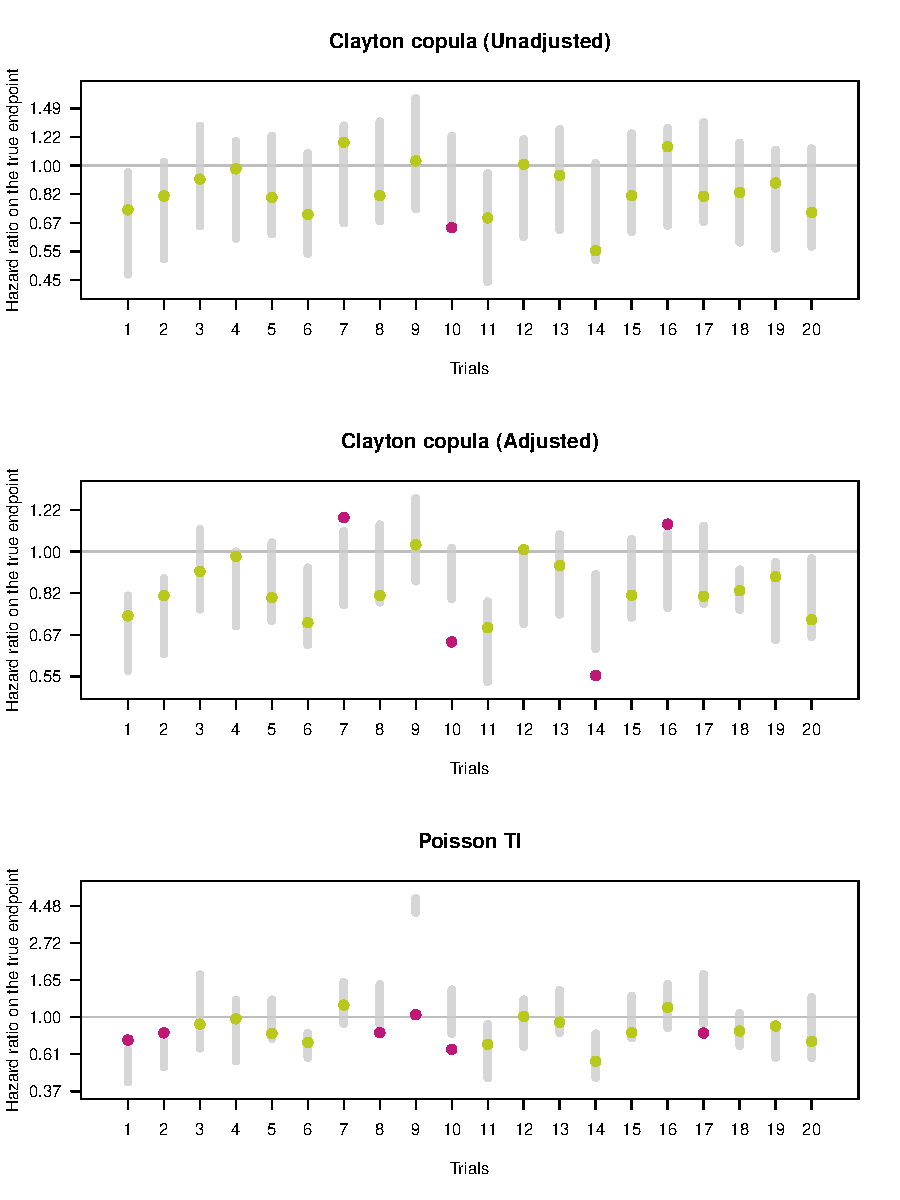
\includegraphics[width=\textwidth]{./loocv-1} \caption[Leave-one-trial-out cross-validation results for the advanced GASTRIC meta-analysis \citep{GASTRIC13}]{Leave-one-trial-out cross-validation results for the advanced GASTRIC meta-analysis \citep{GASTRIC13}. Vertical lines are the 95\% prediction intervals (PI) of the treatment effect on overall survival (OS). Dots are the observed treatment effects on OS (green = within the PI, magenta = out of the PI).}\label{fig:loocv}
\end{figure}
\end{Schunk}




%%%%%%%%%%%%%%%%%%%%%%%%%%%%%%%%%%%%%%%%%%%%%%%%%%%%%%%%%%%%%%%%%%%%%%%%%%%%%%%%
%%%%%%%%%%%%%%%%%%%%%%%%%%%%%%%%%%%%%%%%%%%%%%%%%%%%%%%%%%%%%%%%%%%%%%%%%%%%%%%%
%%%%%%%%%%%%%%%%%%%%%%%%%%%%%%%%%%%%%%%%%%%%%%%%%%%%%%%%%%%%%%%%%%%%%%%%%%%%%%%%
\section{Utilities for data simulation}
%%%%%%%%%%%%%%%%%%%%%%%%%%%%%%%%%%%%%%%%%%%%%%%%%%%%%%%%%%%%%%%%%%%%%%%%%%%%%%%%
%%%%%%%%%%%%%%%%%%%%%%%%%%%%%%%%%%%%%%%%%%%%%%%%%%%%%%%%%%%%%%%%%%%%%%%%%%%%%%%%
%%%%%%%%%%%%%%%%%%%%%%%%%%%%%%%%%%%%%%%%%%%%%%%%%%%%%%%%%%%%%%%%%%%%%%%%%%%%%%%%
Most of the publications that discuss
statistical methods for evaluating failure time surrogate endpoints
do not show simulations till date.
To our knowledge, rare exceptions are those papers by
\cite{BurzykowskiCortinas05, ShiEtal11, RenfroEtal12, Renfro2014, Renfro2015}.

\subsection{Data generation based on a Clayton copula}
The data geration method used by \cite{BurzykowskiCortinas05}
  and by \cite{Renfro2014, Renfro2015} reflects the data generating process 
  underlying the two-step copula model (Sec.~\ref{sec:copulaApp}).

We implemented this approach for the Clayton family (Eq.~(\ref{eq:clayton})),
  which is available using the function \code{simData.cc()}.
This function generates data as follows:
  \begin{itemize}
    \item trial-specific random effects are generated from
      $$
      \binom{m_{S_i}}{m_{T_i}} \sim \mathcal N \left(
      \binom00, \left(\begin{array}{cc}
      \sigma^2_S & \sigma_S\sigma_T\rho_m \\
      \sigma_S\sigma_T\rho_m &  \sigma^2_T
      \end{array}\right)
      \right)
      $$
    \item trial-specific treatment effects are generated from
      $$
      \left(\begin{array}{c} 
      {\alpha_i}\\ {\beta_i}\end{array}\right)
      \sim \mathcal N
      \left(
      \left(\begin{array}{c}
      \alpha\\ \beta\end{array}\right), 
      \left(\begin{array}{cc} 
      d_a^2 &
      d_a d_b{\rho_\text{\tiny trial}} \\
      d_a d_b{\rho_\text{\tiny trial}} &
      d_b^2 \\
      \end{array}\right)
      \right)
      $$
    \item exponentially distributed individual times are simulated
      for $S$, conditionally on the random effects generated before.
      $$
      S_{ij} = -\log(U_{Sij}) / \lambda_{Sij},
      \quad \text{with } 
      \lambda_{Sij} = \exp(\mu_S + m_{S_i} + \alpha_i Z_{ij})
      \text{ and } U_{Sij} \sim U(0,1)
      $$
    \item exponentially distributed individual times are simulated
      for $T\mid S$, conditionally on the random effects generated before
      \textit{and on the value of $S$}
      \begin{align*}
      T_{ij} = -\log(U^\prime_{Tij}) / \lambda_{Tij},
      \quad \text{with }
      \lambda_{Tij} &= \exp(\mu_T + m_{T_i} + \beta_i  Z_{ij}), \\
      U_{Tij}^\prime &= \left[\left(U_{Tij}^{-\theta/(1+\theta)} - 1
      \right) U_{Sij}^{-\theta} + 1 \right]^{-1/\theta}, \text{ and}\\
      U_{Tij} &\sim U(0,1).
    \end{align*}
  \end{itemize}
The details of the arguments of the \code{simData.cc()} function can be 
  obtained using \code{help(simData.cc)}.

\subsection{Data generation based on a mixture of half-normal and exponential random variables}
The data geration method used by \cite{ShiEtal11}
  and by \cite{RenfroEtal12} is based on the results by \cite{Cowles04},
  which showed that a Weibull distribution can be expressed as a scaled mixture
  of half-normal distribution and an exponential distribution
  with unit rate parameter.

This approach, implemented in the function \code{simData.mx()},
  which generates data as follows:
  \begin{itemize}
    \item trial-specific random effects are generated from
      $$
        \binom{m_{S_i}}{m_{T_i}} \sim \mathcal N \left(
        \binom00, \left(\begin{array}{cc}
          \sigma^2_S & \sigma_S\sigma_T\rho_m \\
          \sigma_S\sigma_T\rho_m &  \sigma^2_T
        \end{array}\right)
        \right)
      $$
    \item trial-specific treatment effects are generated from
      $$
        \left(\begin{array}{c} 
        {\alpha_i}\\ {\beta_i}\end{array}\right)
          \sim \mathcal N
          \left(
        \left(\begin{array}{c}
        \alpha\\ \beta\end{array}\right), 
        \left(\begin{array}{cc} 
          d_a^2 &
          d_a d_b{\rho_\text{\tiny trial}} \\
          d_a d_b{\rho_\text{\tiny trial}} &
          d_b^2 \\
        \end{array}\right)
        \right)
      $$
    \item individual half-normal random variables $Y^\ast_{ij}$ 
      are generated from the distribution
      $$
        f(y^\ast) = \frac2{\sqrt{2\pi}} \exp\left(-\frac{{y^\ast}^2}2\right),
        \qquad y^\ast \in \mathbb R_+
      $$
    \item unit rate parameter exponential random variables
      $\Lambda_{Sij}$ and  $\Lambda_{Tij}$ are generated from
      $-\log(U_{Sij})_{Sij}$ and $-\log(U_{Tij})$,
      with $U_{Sij} \sim U(0,1)$ and $U_{Tij} \sim U(0,1)$
    \item exponentially distributed individual times are simulated
      for $S$ and $T$ from
      \begin{align*}
        S_{ij} &= \left(
        Y^\ast_{ij} \sqrt{2\Lambda_{Sij}}
        \right) \exp(\mu_S + m_{S_i} + \alpha_i Z_{ij}), \\
        T_{ij} &= \left(
        Y^\ast_{ij} \sqrt{2\Lambda_{Tij}}
        \right) \exp(\mu_S + m_{T_i} + \alpha_i Z_{ij}).
      \end{align*}
  \end{itemize}
The details of the arguments can be obtained using \code{help(simData.mx)}.

\subsection{Data generation based on mixed proportional hazard models}
In \cite{RotoloPoissurogate}, we also generated data using
  individual random effects to control individual-level surrogacy.
  This approach is implemented in the function \code{simData.re()}
  and generates data as follows:
  \begin{itemize}
    \item trial-specific random effects and 
      trial-specific treatment effects were generated 
      as in the Clayton copula case
    \item individual random effects were generated from
      $u_{ij} \sim \mathcal N(0, \sigma^2)$,
      with $\sigma^2$ depending on the scenario
      (according to the Kendall's $\tau$)
    \item exponentially distributed individual times were simulated
      for $S$ and $T$, conditionally on the random effects generated before.
      We used the inverse transform method, 
      which consists in transforming a uniform random variable
      by means of the inverse of the probability distribution function
      of the random variable to be generated
      \cite[see for instance][\S~2.1.2]{RobertCasella10}
      \begin{align*}
        S_{ij} &= -\log(U_{Sij}) / \lambda_{Sij},
        \quad \text{with } 
        \lambda_{Sij} = \exp(\mu_S + m_{S_i} + \alpha_i Z_{ij} + u_{ij})
        \text{ and } U_{Sij} \sim U(0,1),
        \\
        T_{ij} &= -\log(U_{Tij}) / \lambda_{Tij},
        \quad \text{with }
        \lambda_{Tij} = \exp(\mu_T + m_{T_i} + \beta_i  Z_{ij} + u_{ij})
        \text{ and } U_{Tij} \sim U(0,1). 
      \end{align*}
  \end{itemize}
The details of the arguments can be obtained using \code{help(simData.re)}.


%%%%%%%%%%%%%%%%%%%%%%%%%%%%%%%%%%%%%%%%%%%%%%%%%%%%%%%%%%%%%%%%%%%%%%%%%%%%%%%%
%%%%%%%%%%%%%%%%%%%%%%%%%%%%%%%%%%%%%%%%%%%%%%%%%%%%%%%%%%%%%%%%%%%%%%%%%%%%%%%%
%%%%%%%%%%%%%%%%%%%%%%%%%%%%%%%%%%%%%%%%%%%%%%%%%%%%%%%%%%%%%%%%%%%%%%%%%%%%%%%%
\section*{Acknowledgments}
%%%%%%%%%%%%%%%%%%%%%%%%%%%%%%%%%%%%%%%%%%%%%%%%%%%%%%%%%%%%%%%%%%%%%%%%%%%%%%%%
%%%%%%%%%%%%%%%%%%%%%%%%%%%%%%%%%%%%%%%%%%%%%%%%%%%%%%%%%%%%%%%%%%%%%%%%%%%%%%%%
%%%%%%%%%%%%%%%%%%%%%%%%%%%%%%%%%%%%%%%%%%%%%%%%%%%%%%%%%%%%%%%%%%%%%%%%%%%%%%%%
The present work has been supported
  by the French National Cancer Institute (Institut National du Cancer, INCa),
  Grant SHS 2014-141, and by the Ligue Nationale Contre le Cancer.

% \bibliographystyle{jss}
\bibliography{refs}{}

\appendix
\section{Data poissonization}\label{sec:poisson}
Fitting auxiliary Poisson models for estimating the parameters of 
  a proportional hazard model \citep{Whitehead80, crowtherEtal12}
  needs that data are rearranged in order to provide,
  for each time period, the number of events and the 
  total time passed at risk.
The function \code{poissonize()}in the \pkg{surrosurv} package
  allows to easily perform the necesasry data manipulaton
  easily and quickly.
The core of the function has been derived from the original code
  publicly shared by \cite{Koval}.

The main argument of the \code{poissonize()} function is
  \code{data}, a data frame with columns: 
  \code{id}, the patient identifyier;
  \code{time}, the event/censoring time;
  \code{status}, the event (\code{1}) or censoring (\code{0}) indicator;
  \code{...}, other factors such like the covariables needed
  in the regression model.

The breakpoints between time intervals can be entered in the second argument,
  \code{all.breaks}.
Otherwise, if \code{all.breaks} is not specified,
  one can specify either the width of the time intervals \code{interval.width},
  or their number \code{nInts}
  (used only also if \code{is.null(interval.width)}).

Any other variables to be kept in the poissonized data frame can be entered in
  \code{factors}.
The last argument (\code{compress}) is a logical
  indicating whether the record with the same factor profile
  should be summarized into one record,
  i.~e.\ whether the data should be expressed in a short form.

In the advanced GASTRIC cancer example,
  we first change the column names in order to match the ones needed by
  \code{poissonize()}:
\begin{Schunk}
\begin{Sinput}
R>   gastadv.poi <- gastadv
R>   gastadv.poi$time <- gastadv.poi$timeT / 365.25
R>   gastadv.poi$status <- gastadv.poi$statusT
\end{Sinput}
\end{Schunk}
We fit the proportional hazard model, to which we will compare
  the results of the auxiliary Poisson model.
\begin{Schunk}
\begin{Sinput}
R>   fitcox <- coxph(Surv(time, status) ~ trt, data = gastadv.poi)
R>   cox.base <- basehaz(fitcox, centered = FALSE)
\end{Sinput}
\end{Schunk}
We `possonize' the data over 10 intervals (the default)
  and we fit the auxiliary Poisson model.
\begin{Schunk}
\begin{Sinput}
R>   gastadv.poi <- poissonize(gastadv.poi, nInts = 10, factors = 'trt')
R>   gastadv.poi
\end{Sinput}
\begin{Soutput}
            interval  trt   m  Rt    N
1                  0 -0.5 181 292 1668
2    0.1832128678987 -0.5 180 173 1475
3   0.30921697467488 -0.5 192 149 1288
4  0.435221081451061 -0.5 159 132 1088
5  0.567018480492813 -0.5 154 114  912
6  0.703885010266941 -0.5 156 108  751
7  0.867545516769336 -0.5 157 103  584
8   1.07320739219713 -0.5 143 101  414
9   1.39328678986995 -0.5 117  97  239
10  2.07255030800821 -0.5  60  87   94
11                 0  0.5 216 421 2401
12   0.1832128678987  0.5 221 258 2167
13  0.30921697467488  0.5 213 229 1935
14 0.435221081451061  0.5 247 207 1706
15 0.567018480492813  0.5 237 181 1446
16 0.703885010266941  0.5 225 176 1203
17 0.867545516769336  0.5 228 171  965
18  1.07320739219713  0.5 221 183  715
19  1.39328678986995  0.5 211 205  460
20  2.07255030800821  0.5 117 171  204
\end{Soutput}
\begin{Sinput}
R>   fitpoi <- glm(m ~ -1 + interval + trt + offset(log(Rt)), 
+                 data = gastadv.poi, fam = 'poisson')
\end{Sinput}
\end{Schunk}
The function \code{plotsson()} can be used to draw the survival curves
  (or the instantaneous hazard) estimated by the auxiliary Poisson model:
\begin{Schunk}
\begin{Sinput}
R>   plot(stepfun(cox.base$time[-nrow(cox.base)], 
+                exp(-cox.base$hazard)),
+        ylim = 0:1, xlim = c(0, 5), col = 1, lwd = 2, bty = 'l', yaxs = 'i',
+        do.points = FALSE, verticals = FALSE, xaxs = 'i',
+        main = 'Overall Survival\nAdvanced GASTRIC meta-analysis',
+        xlab = 'Years', ylab = 'Survival probability')
R>   lines(stepfun(cox.base$time[-nrow(cox.base)],
+                exp(-cox.base$hazard * exp(coef(fitcox)['trt']))),
+        col = 2, pch = '', lwd = 2)
\end{Sinput}
\begin{figure}
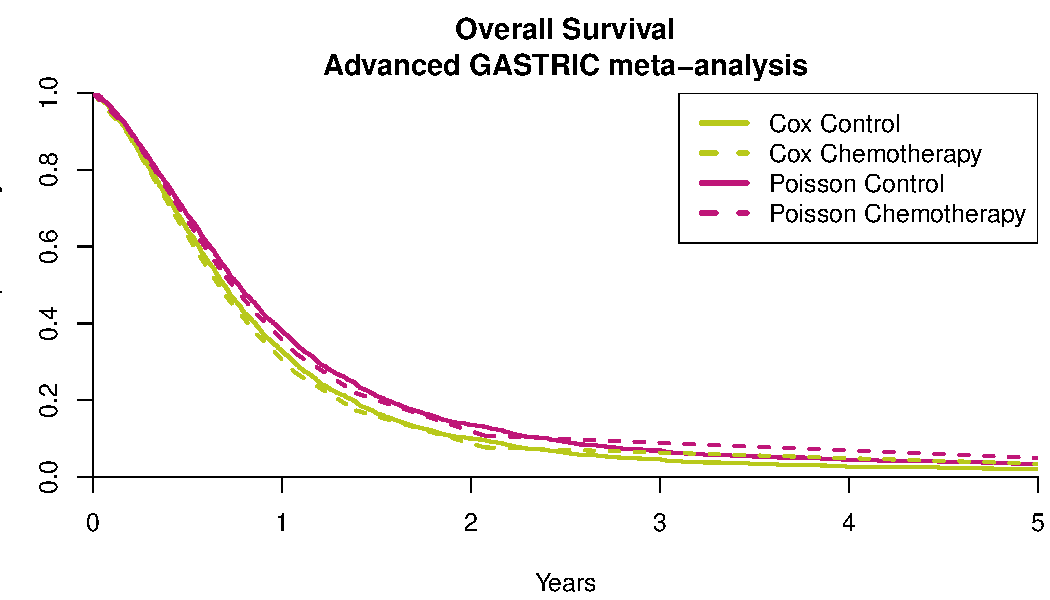
\includegraphics[width=\textwidth]{./poissonize-1} \caption{Overall survival curves in the advanced GASTRIC meta-analysis \citep{GASTRIC13}. \textbf{(a)} Comparison between the survival probability obtanied using the Breslow estimator in the Cox model (solid lines) and those obtained using the auxiliary Poisson model (dashed lines). \textbf{(b)} Piecewise constant hazard estimated by the auxiliary Poisson model}\label{fig:poissonize}
\end{figure}
\end{Schunk}
The treatment effect estimated by the Cox model is
  \ensuremath{-0.14} (SE = 0.03), 
  and it is of 
  \ensuremath{-0.14} 
  (SE = 0.03)
  when using the auxiliary Poisson model.

\end{document}
